%%%%%%%%%%%%%%%%%%%%%%%%%%%%%%%%%%%%%%%%%%%%%%%%%%%%%
\chapter{Semi-discrete Optimal Transport}
The Damped Newton algorithm, hereafter DA, developed by M\'{e}rigot et al. \cite{Merigot2017} solves a semi-discrete Monge-Amp\`{e}re type optimal transport problem. It's efficiency in exploiting the properties of sparse matrices and linear convergence \cite{Merigot2017} make it practical for implementation in the solution for equations \ref{EadyGC}. Further detail describing the application of the algorithm in the solution to the Eady Model is given in chapter \ref{algorithm}. In this chapter an overview of semi-discrete optimal transport is given using definitions given in \cite{Kitagawa2016, Merigot2017} as well as a comparison to the energy minimisation to which it is applied. A rigorous proof of the formulation of \ref{EadyModel} as a Monge-Amp\`{e}re type optimal transport problem is given in Cullen, 2006 \cite{Cullen2006a}.
\section{Semi-discrete Optimal Transport}
\begin{figure}[h]
	\centering
	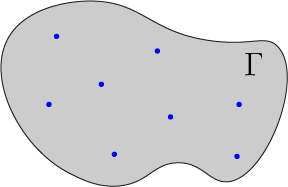
\includegraphics[width=5.5cm]{project/probmeasure}
	\caption[Semi-discrete Optimal Transport]{A discrete (target) set $Y \subseteq \mathbb{R}^2$ represented by blue points in a compact domain (source) $\Gamma \subseteq \mathbb{R}^2 $}
	\label{fig:probmeasure}
\end{figure}
Optimal transport problems describe the problem of finding a map between two sets, a target set and a source set, each with an associated density, in such a way that the "cost" associated with the mapping is minimised. In semi-discrete optimal transport the target set is a finite set.\\
\linebreak
In Kitagawa et al. \cite{Kitagawa2016} a wonderful analogy with travel distance to bakeries in a city is made, where the source set is considered as a city and the discrete target set is the locations of bakeries in the city. In this report the problem will be explained in the context in which it will subsequently be implemented. Namely, the source set is the domain $\Gamma$, the physical space described in section \ref{Chapter3} and the target set, the set of points in geostrophic space. The optimal transport problem finds a partition of the domain, up to sets of measure zero, such that every point in a region of the partion is closest to the point at the centre of that region. In this analogy the cost being minimised is the travel distance to the point $\bm{Y}_i$, $c(\bm{x},\bm{Y}_i) = \|\bm{x}-\bm{Y}_i \|^2$, where $\bm{x} \in \Gamma$. This is illustrated in figure \ref{fig:laguerrediagram0w}  below
\begin{figure}[h]
	\centering
	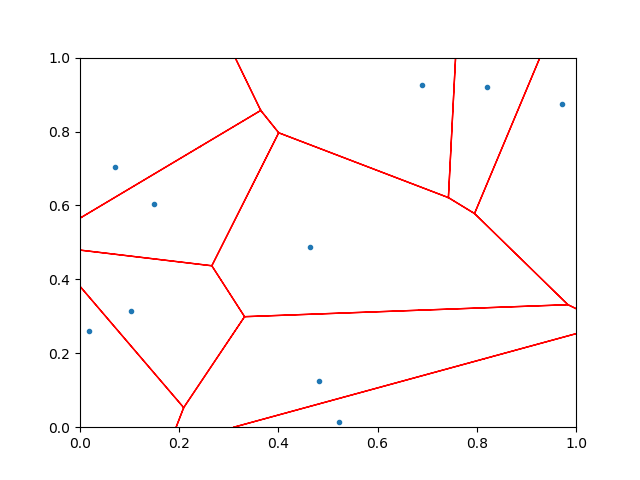
\includegraphics[width=8cm]{project/laguerre_diagram_0w}
	\caption[The partitioning of a Domain]{The image showing how a domain would be divided into areas based on minimising distance to the blue points. This is a Voronoi tesselation of the domain $\Gamma$ based on the minimisation of $c(\bm{x},\bm{Y_i})$}
	\label{fig:laguerrediagram0w}
\end{figure}
\\
To put this into a more rigorous mathematical setting, given a domain  $\Gamma\subseteq \mathbb{R}^2$ and discrete set of $N$ points $Y = \left\lbrace \bm{Y}_i = (X_i,Z_i), \quad 1\leq i \leq N \right\rbrace  \subset \mathbb{R}^2$,
\begin{definition}
	\textbf{Source measure} \\ Defined on the domain $\Gamma$. $\mu(A) = \textrm{Area}(\Gamma)^{-1}\int_A \ dxdz$, $A \subseteq \Gamma$. Note this defines a probability measure with a uniform probability density on $\Gamma$.
\end{definition}
\begin{definition}
	\textbf{Target measure} \\Defined on $\mathbb{R}^2$ $\sigma((X,Z)) = \sum_{i=1}^{N}\sigma_i \delta\left(\bm{Y}-\bm{Y}_i\right)$, with finite support on $\mathbb{R}^2$. Note this defines a discrete probability measure when $\sigma(\mathbb{R}^2) = 1$, for appropriate choice of $\sigma_i$.
	\label{target measure}
\end{definition}
\begin{definition}
	\textbf{Voronoi Cells} \\ The regions enclosed by the red lines and boundaries of the domain in \ref{fig:laguerrediagram0w} are defined as Voronoi cells, $\text{Vor}(\bm{Y}_i) := \left\lbrace \bm{x} \in \Gamma \; \text{st} \; \forall \ Y_j \in Y \; c(\bm{x},\bm{Y}_i) \leq c(\bm{x},\bm{Y}_j) \right\rbrace$. The diagram is referred to as a Voronoi tesselation.
\end{definition} 
\begin{definition} 
	\textbf{Transport map} \\ $T: \Gamma \rightarrow Y$ between the source measure $\mu$ and the target measure on $Y$, $\mu$ if $T_{\#}\mu = \sigma$.\\
\end{definition}
\begin{definition}
	\textbf{Pushforward} of a measure $\mu$ by a map $T: \Gamma \rightarrow Y$ is $T_{\#}\mu = \sum_{\bm{Y}_i \in Y} \mu \left( T^{-1}(\bm{Y}_i) \right) \delta(\bm{Y}-{\bm{Y}_i})$, the sum of the measures of the sets mapped to the points $\bm{Y}_i$ under $T$
\end{definition}
From these definitions we can see that the optimal transport map is given by,
\begin{equation}
	T(\bm{x}) = \arg\min_{\bm{Y}_i\in Y}\left(c(\bm{x},\bm{Y}_i)\right) \iff \sigma(\bm{Y}_i) = \mu\left(\text{Vor}(\bm{Y}_i)\right)
\end{equation}
\section{Laguerre Cells and the Inclusion of weights}
 \begin{figure}[h]
	\centering
	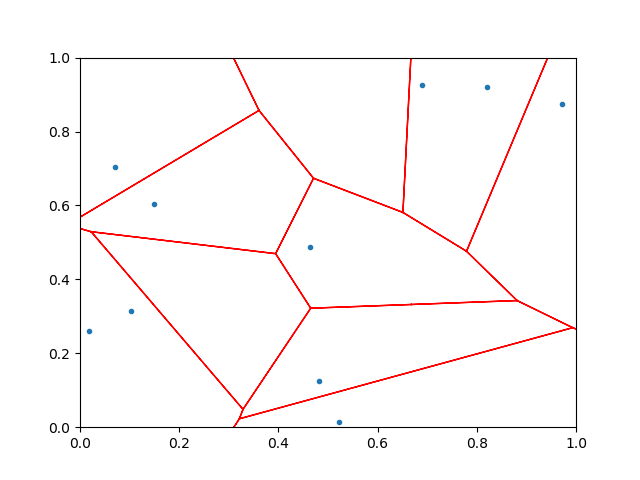
\includegraphics[width=8cm]{project/laguerre_diagram_OTw}
	\caption[Laguerre diagram produced by finding weights using DA for optimal transport]{Given a uniform source and target density the Laguerre diagram produced by finding weights using DA for optimal transport}
	\label{fig:laguerrediagramotw}
\end{figure}
Considering again figure \ref{fig:laguerrediagram0w} it is clear that if the density across the domain $\Gamma$ is uniform the distribution of area corresponding to each bakery is certainly not. For example, the Voronoi cells at the top right of the diagram in figure \ref{fig:laguerrediagram0w} are much larger in area than those in the centre of the diagram. This raises the problem of finding a way to create a partition such that each cell has the same area. This is done by introducing an additional$\ $\textquotedblleft weight\textquotedblright$\ $argument to the cost. We denote the weights by $\psi_i = \psi\left(\bm{Y}_i\right) \in \mathbb{R}$. In the case of the bakeries the weights might represent the price of bread at a specific bakery. For this we introduce the notion of Laguerre cells.\\
\begin{definition}
	\textbf{Laguerre Cells}\\
	 The regions enclosed by the red lines and boundaries of the domain in figure \ref{fig:laguerrediagramotw},  $\text{Lag}_{\bm{Y}_i}(\psi) := \left\lbrace \bm{x} \in \Gamma \; \text{st} \; \forall \ \bm{Y}_j \in Y \; c(\bm{x},\bm{Y}_i) + \psi(\bm{Y}_i) \leq c(\bm{x},\bm{Y}_j) + \psi(\bm{Y}_j) \right\rbrace$
	 \label{def: laguerre cell}
\end{definition}
In this case, the optimal transport map is given by \\
$T_\psi: x \rightarrow \text{argmin}_i\| x - y_i \|^2 + \psi_i$, where $\psi_i$ is a family of weights on $Y$ \cite{Merigot2017}.\\
\linebreak
 The problem is then finding the weights $\psi_i$ associated to the points $\bm{Y}_i$ such that $\mu (\text{Lag}_{\bm{Y}_i}(\psi)) = \sigma(\bm{Y}_i) = \sigma_i$. The Damped Newton's Algorithm from M\'{e}rigot, Meyron and Thibert (2017) \cite{Merigot2017} finds such $\psi_i$.
 \\
 \linebreak 
 Supposing that both the source density and target density are uniform, (ie) in definition \ref{target measure} the Laguerre cells as found by the DA code developed in \cite{Merigot2017} are shown in figure \ref{fig:laguerrediagramotw}. The Laguerre diagram highlights the fact that the densities are both specified to be uniform probability densities. In figure \ref{fig:laguerrediagram0w} the target density was not specified. This means that points are not necessarily interior to their corresponding Laguerre cells, however the cells have equal area. The cells in this case are the Laguerre cells defined above, and the weights that define the optimal transport map was found by \cite{Merigot2017} as
 \begin{equation*}
 T(x) = \arg\min_{\bm{Y}_i\in Y}\left(c(\bm{x},\bm{Y}_i) + \psi_i\right)
 \end{equation*}
For the remainder of this report we will consider cases where both the source density and target density are uniform and the quadratic cost function is,
\begin{equation*}
	c(\bm{x},\bm{Y}_i) = \| \bm{x} - \bm{Y}_i \|^2
\end{equation*}
\section{Applying semi-discrete optimal transport to solving the semi-geostrophic equations}
As shown in \cite{Cullen2006a} equations \ref{EadyModel} can be recast as an optimal transport problem using the transformation to geostrophic co-ordinates introduced by Hoskins \cite{Hoskins1975}. In this section we outline how DA is applied to equations \ref{EadyModel}.
\\
\linebreak
The optimal transport problem considered in the frontogenesis problem is the minimisation of the energy, restated from equation \ref{energy}
\begin{equation}
E = f^2 \iint \frac{1}{2}\left(X-x\right)^2 - Z\left(z - H/2\right)\textrm{d}x\textrm{d}z
\end{equation}
as shown by Lemma \ref{energy lemma} this is equivalent to minimising \ref{energy1},
\begin{equation}
E = \frac{f^2}{2} \iint \left(\left(X-x\right)^2 + \left(Z - z\right)^2\right)\textrm{d}x\textrm{d}z
\end{equation}
Considering the geostrophic co-ordinates as the target set of finite set of points for the optimal transport problem from the domain $\Gamma = [-L,L] \times [0,H]$. The DA Algorithm finds the weights such that the area of each Laguerre cell is preserved. Physically, this amounts to the condition that the volume is conserved.
\section{Extension for Periodic Boundary Conditions}
As stated in Chapter \ref{governingequations} in the model for frontogenesis boundary conditions consider periodicity in $x$. This must be accounted for in the implementation of the Damped Newton Algorithm.
\\
\linebreak
This inclusion of periodic boundary conditions allows Laguerre cells to cover areas over the right and left boundaries. This means that the Laguerre edges must be continuous across the boundaries if copies of the Laguerre diagram were placed on each boundary. The Laguerre cells must have the same mass, for example, in figure \ref{fig:laguerrediagramotpw} below the top right cell extends to the left of the domain. The sum of the areas of each component of the cell must be the same as a cell in the centre of the diagram. The area of each cell remains the same as in \ref{fig:laguerrediagramotw} however the boundaries of the Laguerre cells are continuous across the left and right boundaries of the domain.
\begin{figure}[h]
	\centering
	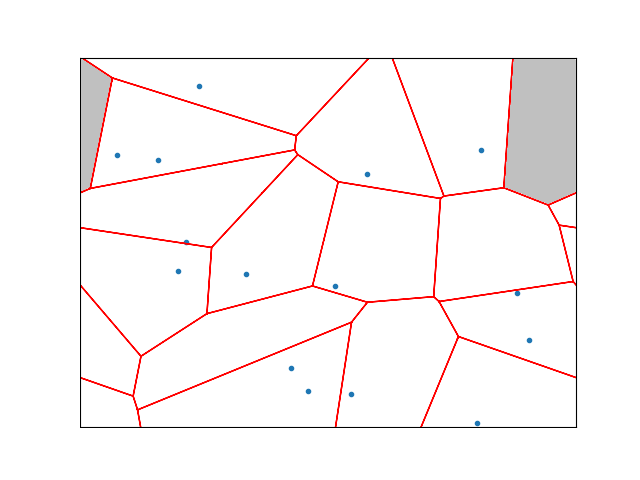
\includegraphics[width=8cm]{project/laguerre_diagram_OTPw}
	\caption[Optimal Transport with Periodic Boundary Conditions]{The solution to the optimal transport of the same points shown in figure \ref{fig:laguerrediagramotw}, however with the density initialised with periodic boundary conditions in $x$. The area shaded in grey represents a single Laguerre cell.}
	\label{fig:laguerrediagramotpw}
\end{figure}
\subsection{Definitions of Mass with Periodic Boundary Conditions}
\begin{figure}[h]
	\centering
	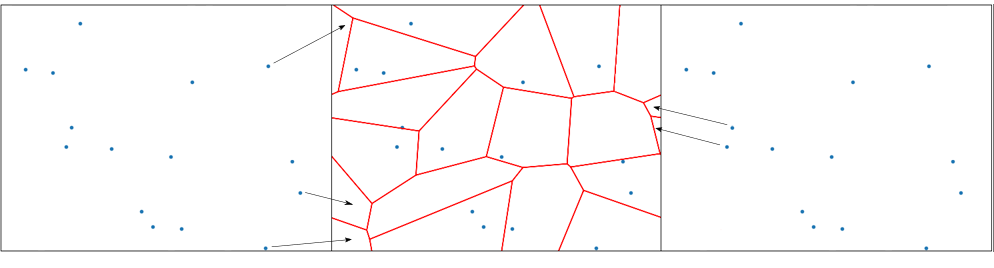
\includegraphics[width=1\linewidth]{project/laguerre_diagram_OTPw_periodic}
	\caption[Periodic boundary conditions with 'ghost' points]{The image above shows how the Laguerre diagram for periodic boundary conditions is created with 'ghost' points on either side of the domain. Arrows show where ghost points contribute to Laguerre cells of positive mass in the domain $\Gamma$}
\end{figure}

\comments{include the definition of mass of a cell and a better written description of the partition given by a laguerre diagram (tesselation/zero measure sets)}
\comments{include definition of the fundamental domain}
\subsection{Mapping to the Fundamental Domain}
Under the geostrophic transformation \ref{transformation} and also in time-stepping points in geostrophic space it is possible for points to travel exterior the boundaries of the domain $\Gamma$. In the $x$ direction the boundary conditions imposed are periodic. If points are mapped so that their $x$-co-ordinates are exterior to the interval $[-L,L]$, they can be mapped to the domain $\Gamma$, the \textquoteleft fundamental domain\textquoteright, using the periodicity, without affecting the result. \comments{better phrasing please} In fact, in the implementation of DA this is necessary at every time step to ensure that the mass of cells remains positive. This is implemented by the function \textquoteleft to\_fundamental\_domain\textquoteright \ adapted from DA \cite{Merigot2017a} to treat periodic boundary conditions in $x$. An example of this is shown in figure \ref{fundamental domain} below, where the fundamental domain being considered is $[0,1]\times[0,1]$.
\begin{figure}[h!]
	\centering
	\subfloat[]{{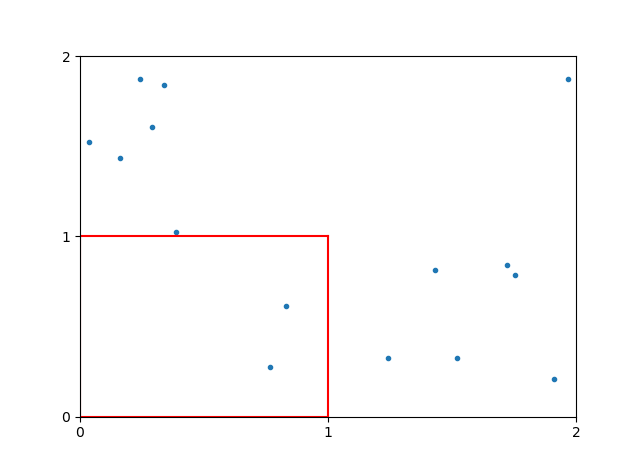
\includegraphics[width=7cm]{project/fund_domain_out}\label{out of fund domain}}}
	\subfloat[]{{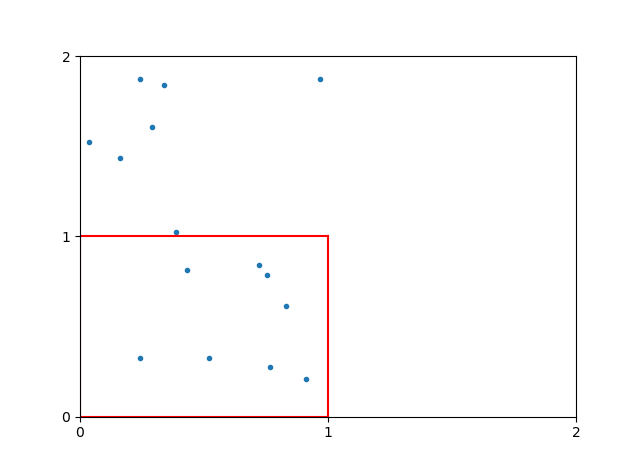
\includegraphics[width=7cm]{project/fund_domain_in}\label{in fund domain}}}
	\caption{Plots of a random set of points initialised in $[0,2]\times[0,2]$ before (a) and after (b) being mapped to the fundamental domain $[0,1]\times[0,1]$}
	\label{fundamental domain}
\end{figure}
\\
To explain this rigorously, we consider the domain described by $[x_0,y_0] \times [x_1,y_1]$. Since we are only considering periodic boundary conditions in $x$, only the $x$ co-ordinates will be mapped. 
\\
The mapping is performed by first finding the distance of the point from the left boundary of the domain as a ratio of the width of the domain. This is then added to left bound to give a value for $x$, $\tilde{x}$ that is in the fundamental domain. 
\begin{equation*}
	\begin{aligned}
		X &= x - \floor*{\frac{x - x_0}{x_1 - x_0}}\\
		\tilde{x} &= x_0 + (x_1 - x_0)X
	\end{aligned}
\end{equation*}
This is implemented as:
\comments{insert to\_fundamental\_domain code}
%%%%%%%%%%%%%%%%%%%%%%%%%%%%%%%%%%%%%%%%%%%%%%%%%%%%%
\chapter{A Numerical Solution to the Eady Model for Frontogenesis \label{algorithm}}
In this section the numerical implementation including the use of the Damped Newton Algroithm developed by \cite{Merigot2017} is explained in detail. 
Restating the problem, we are solving the semi-geostrophic equations \ref{EadyModel} over the domain $\Gamma := [-L,L] \times [0,H]$.
\begin{equation*}
	\begin{aligned}
		-fv_g + \frac{\partial \varphi}{\partial x} = 0,\\
		\frac{Dv_g}{Dt} + fu -\frac{Cg}{\theta _0}\left(z-H/2\right) = 0,\\
		\frac{D\theta'}{Dt} - Cv_g = 0,\\
		\frac{\partial \varphi}{\partial z} - g\frac{\theta'}{\theta_0} = 0,\\
		\nabla \cdot \bm{u} = 0.
	\end{aligned}
\end{equation*}
With boundary conditions:
\vspace{-\topsep}
\begin{itemize}
	\setlength{\parskip}{0pt}
	\setlength{\itemsep}{0pt}
	\item Rigid lid condition $w = 0$ on $z = 0, H$
	\item Periodic boundary conditions in $x$
\end{itemize}
\vspace{-\topsep}
Together with a baroclinic instability described by \ref{thetap} as
\begin{equation}
\theta' = \frac{N^2\theta_0 z}{g} + B\sin\left(\pi\left(x/L + z/H\right)\right)
\end{equation}
The steps involved in solving the Eady Model for frontogenesis described above are detailed below,
\begin{description}
	\setlength{\parskip}{0pt}
	\setlength{\itemsep}{0pt}
	\item[Step 1] Initialise a set of points in physical space
	\item[Step 2] Transform physical points to Geostrophic space using the co-ordinate transformation given in \ref{transformation}, and map to fundamental domain $\Gamma$.
	\item[Step 3] Given the points in geostrophic space the weights which define the Laguerre cells in the physical domain are calculated using the Damped Newton Algorithm.
	\item[Step 4] The equations are now time stepped from the transformed momentum equations \ref{EadyGC} 
	\begin{equation*}
		\begin{aligned}
			\frac{\mathrm{D}X_{n}}{\mathrm{D}t} -\frac{Cg}{f\theta _0}\left(\tilde{z}_n-H/2\right) = 0 \\
			\frac{\mathrm{D}Z_{n}}{\mathrm{D}t} - \frac{Cg}{f\theta_0}\left(X_n - \tilde{x}_n\right) = 0
		\end{aligned}
	\end{equation*}
	Where $X_n, Z_n$ represent the geostrophic points at the current time step, and $\tilde{x}_n,\tilde{z}_n$ represent the centroids of the Laguerre cells. In this project both a Forward-Euler scheme and Heun's method have been used for time-stepping.
	\item[Step 5] The geostrophic points are now replaced with $X_{n+1}, Z_{n+1}$ and steps 3 and 4 are repeated until the final time is reached.
\end{description}
\section{Initialisation of Points in Geostrophic Space \label{Initpoints}}
Given a finite set of equidistant points in the physical domain $\Gamma$, the points are transformed to geostrophic space using
\begin{equation}
X = x + \frac{v_g}{f}, \qquad Z = \frac{g\theta'}{f^2\theta_0}
\label{geostrophictransformation}
\end{equation}
This requires the form of $\theta'$ given by \ref{thetap} from this $v_g$ can be deduced using the following equations from \ref{EadyModel},
\begin{equation}
	\begin{aligned}
		\frac{\partial \varphi}{\partial z} - \frac{g \theta'}{\theta_0} = 0\\
		\frac{\partial \varphi}{\partial x} - fv_g = 0
	\end{aligned}
\label{findingvg}
\end{equation}
using the boundary condition $\int_{0}^{H}\varphi(x,z)\text{ d}z = 0$
Integrating the first equation in $z$,
\begin{equation*}
	\begin{aligned}
	\frac{\partial \varphi}{\partial z} = \frac{g \theta'}{\theta_0} = N_0^2z + \frac{Bg}{\theta_0}\sin\left(\pi\left(\frac{x}{L}+\frac{z}{H}\right) \right)\\
	\varphi = \frac{N_0^2z^2}{2} - \frac{BgH}{\theta_0\pi}\cos\left(\pi\left(\frac{x}{L}+\frac{z}{H}\right)\right) + F(x)
	\end{aligned}
\end{equation*}
Applying the boundary condition to determine $F(x)$,
\begin{equation*}
	\begin{aligned}
	\int_{0}^{H}\varphi \text{ d}z = \left[ \frac{N_0^2z^3}{6} - \frac{BgH^2}{\theta_0\pi^2}\sin\left(\pi\left(\frac{x}{L}+\frac{z}{H}\right) \right) + F(x)z\right]_{0}^{H} = 0
	\end{aligned}
\end{equation*}
Using $\sin\left(\frac{\pi x}{L}+\pi\right) = -\sin\left(\frac{\pi x}{L}\right)$,
\begin{equation*}
\begin{aligned}
 0 & =\frac{N_0^2H^3}{6} - \frac{BgH^2}{\theta_0\pi^2}\sin\left(\frac{\pi x}{L}+\pi\right)+ \frac{BgH^2}{\theta_0\pi^2}\sin\left(\frac{\pi x}{L}\right) + F(x)H\\
 0 & =\frac{N_0^2H^3}{6} + \frac{2BgH^2}{\theta_0\pi^2}\sin\left(\frac{\pi x}{L}\right) + F(x)H
\end{aligned}
\end{equation*}
This gives $F(x)$ as,
\begin{equation*}
	F(x) = -\frac{N_0^2H^2}{6} - \frac{2BgH^2}{\theta_0\pi^2}\sin\left(\frac{\pi x}{L}\right)
\end{equation*}
and consequently $\varphi$ as,
\begin{equation}
	\varphi(x,z) = \frac{N_0^2z^2}{2} - \frac{BgH}{\theta_0\pi}\cos\left(\pi\left(\frac{x}{L}+\frac{z}{H}\right)\right)-\frac{N_0^2H^2}{6} - \frac{2BgH}{\theta_0\pi^2}\sin\left(\frac{\pi x}{L}\right)
\end{equation}
Using the second of equations \ref{findingvg} $v_g$ is found as,
\begin{equation}
	v_g = \frac{BgH}{f\theta_0L}\cos\left(\pi\left(\frac{x}{L}+\frac{z}{H}\right)\right)- \frac{2BgH}{f\theta_0\pi}\sin\left(\frac{\pi x}{L}\right)
	\label{vg}
\end{equation}
Together with $\theta'$ given by \ref{thetap} this expression for $v_g$ can be used to determine $X$ and $Z$ in geostrophic co-ordinates through the transform \ref{geostrophictransformation}.
\begin{figure}[h]
	\centering
	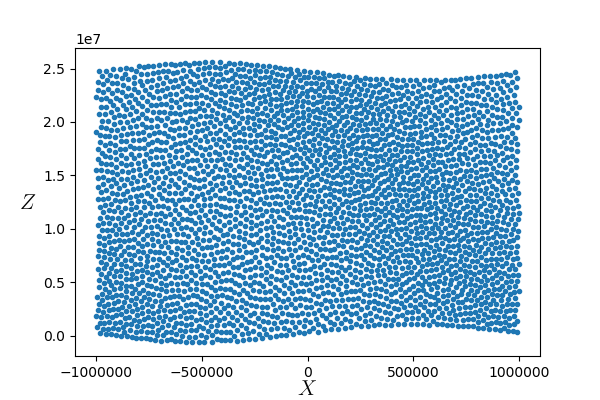
\includegraphics[width=7cm]{project/gpoints}
	\caption[Plot of Points in Geostrophic Space]{Plot of points in geostrophic space, transformed from a random set of points in $\Gamma := [-L,L] \times [0,H]$ using \ref{transformation} with $v_g$ as defined in \ref{vg}}
	\label{fig:gpoints}
\end{figure}

\section{Choice of Initial Weights \label{Initweights}}
The Laguerre diagram of this set of points shown in figure \ref{fig:gpoints} with zero weights would define Laguerre cells exterior to $\Gamma$. These cells will have zero \textquotedblleft mass \textquotedblright in the domain $\Gamma$. Physical intuition tells us that given the rigid lid and periodic boundary conditions points would physically not be able to leave the domain. However, thinking of fluid particles as the centroids of Laguerre cells, a cell outside the domain would represent a fluid particle on the exterior of the domain. This also poses a problem with respect to the implementation of DA, as emphasised in \cite{Merigot2017}, as it requires $\mu\left(\text{Lag}_{y_i}(\psi)\right)$ to be a monotonic function of $\psi = (\psi(y_1),...,\psi(y_N))$ where $N$ is the number of points initialised in $\Gamma$. According to \cite{Merigot2017} this occurs near points where the Laguerre cells contain positive mass over $\Gamma$.\\
\linebreak
Fortunately, a solution is provided in \cite{Merigot2017}. Proposition 25 in the paper proves that if the initial weights are given by,
\begin{equation*}
	\psi_i^0 = d\left(\bm{Y}_i,\Gamma\right)^2
\end{equation*}
where $\bm{Y}_i = \left(X_i,Z_i\right)$ are the points in geostrophic space. Since the domain is rectangular vertical distance from the point to the upper or lower boundary of the domain. The boundaries, given by $z=0$ and $z = H$ are also perturbed to guarantee strict positivity of the mass of the Laguerre cells, 
\begin{equation}
\psi_i^0 = \begin{cases}
\left(Z_i - 0.9H\right)^2, & Z_i > 0.9H \\
\left(Z_i - 0.1H\right)^2, & Z_i < 0.1H
\end{cases}
\label{weights}
\end{equation}
\comments{Address disparity with paper '-' sign - convention used in paper for finding Laguerre cells different to code?}
The Damped newton algorithm, DA, is initialised with the the geostrophic points and weights given by \ref{weights}. The algorithm outputs weights that give Laguerre cells with equal mass over the periodic domain.
\section{Time Stepping \label{timestep}}
Once the initial points and weights have been set up, it remains to find the geostrophic points at the next time step, using equations \ref{EadyGC}.
\subsection{Forward-Euler Scheme}
The numerical solution to equations \ref{EadyModel} developed follows a Lagrangian framework, thus it is justified to treat the material derivative $\frac{\mathrm{D } }{\mathrm{D} t}$ as a full derivative $\frac{\mathrm{d }}{\mathrm{d} t}$, in this sense we will develop prognostic scheme using the equations,
	\begin{equation*}
	\begin{aligned}
	\frac{\mathrm{d}X}{\mathrm{d}t} -\frac{Cg}{f\theta _0}\left(\tilde{z}-H/2\right) = 0 \\
	\frac{\mathrm{d}Z}{\mathrm{d}t} - \frac{Cg}{f\theta_0}\left(X - \tilde{x}\right) = 0
	\end{aligned}
	\end{equation*}
Applying a Forward-Euler scheme \cite{Griffiths2010} for time-stepping given by,
\begin{equation}
	\begin{aligned}
	t^{n+1} &= t^n + h\\
	Z_i^{n+1} &= Z_i^n + \frac{hCg}{f\theta_0}\left(X_i^n-\tilde{x}_i^n\right)\\
	X_i^{n+1} &= X_i^n + \frac{hCg}{f\theta_0}\left(\tilde{z}_i^n-H/2\right)
	\end{aligned}
\end{equation}
where $\tilde{x}_i^n,\tilde{z}_i^n$ represent the centroids of the Laguerre cells given by equations \ref{centroids} using $X_i^n,Z_i^n$ and corresponding weights given by the optimal transport algorithm (DA),
\begin{equation}
	\tilde{x}_i^n = \frac{\int_{\mathrm{Lag}_{\bm{Y}_i^n}(\psi)} x \  \mathrm{d}x \mathrm{d}z}{\int_{\mathrm{Lag}_{\bm{Y}_i^n}(\psi)} \mathrm{d}x \mathrm{d}z}, \qquad
	\tilde{z}_i^n = \frac{\int_{\mathrm{Lag}_{\bm{Y}_i^n}(\psi)} z \ \mathrm{d}x \mathrm{d}z}{\int_{\mathrm{Lag}_{\bm{Y}_i^n}(\psi)} \mathrm{d}x \mathrm{d}z}
	\label{centroids}
\end{equation}
Before the next iteration of the time-step the points $X_i^{n+1}, Z_i^{n+1}$ are mapped back to the fundamental domain.
\subsection{Heun's Method}
For comparison and to test convergence the time-stepping was also implemented using Heun's method \cite{Griffiths2010}.
\begin{equation}
	\begin{aligned}
	t^{n+1} &= t^{n} + h, \quad
	\hat{Z}_i^{n+1} = Z_i^n +  \frac{hCg}{f\theta_0}\left(X_i^n-\tilde{x}_i^n\right), \quad
	\hat{X}_i^{n+1}  = X_i^n +  \frac{hCg}{f\theta_0}\left(\tilde{z}_i^n-H/2\right)\\
	Z_i^{n+1} &= Z_i^n + \frac{h}{2}\left( \frac{Cg}{f\theta_0}\left(X_i^n-\tilde{x}_i^n\right)+ \frac{Cg}{f\theta_0}\left(\hat{X}_i^{n+1}-\hat{x}_i^{n+1}\right)\right)\\
	X_i^{n+1}  &= X_i^n + \frac{h}{2}\left( \frac{Cg}{f\theta_0}\left(\tilde{z}_i^n-H/2\right) + \frac{Cg}{f\theta_0}\left(\hat{z}_i^{n+1}-H/2\right)\right)
	\end{aligned}
\end{equation}
Where again, $\hat{x}_i^n$ and $\hat{z}_i^n$ represent the centroids of the Laguerre cells given using \ref{centroids} and $\hat{X}_i^{n+1},\hat{Z}_i^{n+1}$ with corresponding weights given by the optimal transport algorithm DA.

\comments{why not higher order time-step method? Limited by OT solver - 2nd order?}
\comments{include map back to fundamental domain explanation and why this isn't done for centroids}
A comparison of results using Heun's method and the forward-Euler scheme for timestepping is detailed in Chapter \ref{results}.
\section{Visualising the Output \label{plotting}}
Given the Geostrophic points and the associated weights which solve the optimal transport problem a Laguerre diagram satisfying \ref{def: laguerre cell} can be constructed. In the Monge-Amp\`{e}re library of DA \cite{Merigot2017,Merigot2017a} there is a function to rasterize a Laguerre diagram to a pixelated image, with Laguerre cells coloured according to the value of a particular variable.\\
\linebreak
For example, in the images below the Laguerre cells are coloured according to the value of $\theta '$ given by, $\theta ' = \frac{f^2\theta_0 Z}{g}$
%%%%%%%%%%%%%%%%%%%%%%%%%%%%%%%%%%%%%%%%%%%%%%%%%%%%%
